% Fig. 1: HEAL-GTN architecture (vector, Times 8 pt). Compile with pdflatex.
\documentclass[10pt,border=1pt]{standalone}
\usepackage{mathptmx}
\usepackage{amsmath}
\usepackage{tikz}
\usetikzlibrary{positioning,arrows.meta,fit,calc,backgrounds}
\begin{document}
\footnotesize
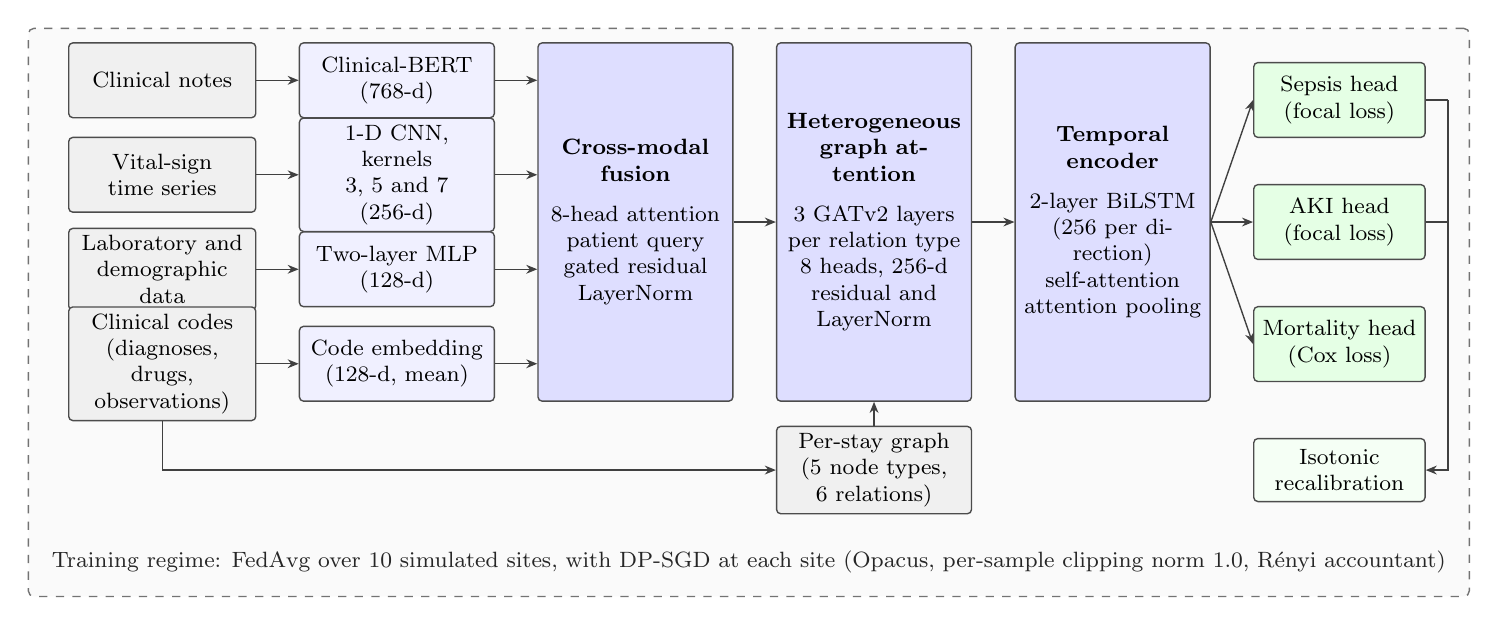
\begin{tikzpicture}[
  font=\footnotesize,
  >={Stealth[length=4pt,width=3.2pt]},
  box/.style={draw=black!70, line width=0.5pt, rounded corners=1.5pt, align=center,
              inner sep=2.5pt, minimum height=0.95cm},
  inp/.style={box, fill=black!6, text width=2.20cm},
  enc/.style={box, fill=blue!6, text width=2.30cm},
  core/.style={box, fill=blue!13, text width=2.30cm, minimum height=4.55cm},
  head/.style={box, fill=green!10, text width=2.00cm},
  arr/.style={->, draw=black!75, line width=0.5pt}
]
% ---------------- inputs
\node[inp] (n1) at (0,  1.80) {Clinical notes};
\node[inp] (n2) at (0,  0.60) {Vital-sign\\ time series};
\node[inp] (n3) at (0, -0.60) {Laboratory and\\ demographic data};
\node[inp] (n4) at (0, -1.80) {Clinical codes\\ (diagnoses, drugs,\\ observations)};
% ---------------- encoders
\node[enc] (e1) at (2.98,  1.80) {Clinical-BERT\\ (768-d)};
\node[enc] (e2) at (2.98,  0.60) {1-D CNN, kernels\\ 3, 5 and 7 (256-d)};
\node[enc] (e3) at (2.98, -0.60) {Two-layer MLP\\ (128-d)};
\node[enc] (e4) at (2.98, -1.80) {Code embedding\\ (128-d, mean)};
\foreach \i in {1,2,3,4} { \draw[arr] (n\i.east) -- (e\i.west); }
% ---------------- core blocks
\node[core] (fu) at (6.01, 0) {\textbf{Cross-modal}\\ \textbf{fusion}\\[5pt] 8-head attention\\ patient query\\ gated residual\\ LayerNorm};
\node[core] (gn) at (9.04, 0) {\textbf{Heterogeneous}\\ \textbf{graph attention}\\[5pt] 3 GATv2 layers\\ per relation type\\ 8 heads, 256-d\\ residual and\\ LayerNorm};
\node[core] (tm) at (12.07, 0) {\textbf{Temporal}\\ \textbf{encoder}\\[5pt] 2-layer BiLSTM\\ (256 per direction)\\ self-attention\\ attention pooling};
\foreach \i in {1,2,3,4} { \draw[arr] (e\i.east) -- (e\i.east -| fu.west); }
\draw[arr] (fu.east) -- (gn.west);
\draw[arr] (gn.east) -- (tm.west);
% graph builder fed by codes
\node[box, fill=black!6, text width=2.30cm, minimum height=0.8cm] (gb) at (9.04, -3.15)
  {Per-stay graph\\ (5 node types,\\ 6 relations)};
\draw[arr] (n4.south) |- (gb.west);
\draw[arr] (gb.north) -- (gn.south);
% ---------------- heads
\node[head] (h1) at (14.95,  1.55) {Sepsis head\\ (focal loss)};
\node[head] (h2) at (14.95,  0.00) {AKI head\\ (focal loss)};
\node[head] (h3) at (14.95, -1.55) {Mortality head\\ (Cox loss)};
\foreach \i in {1,2,3} { \draw[arr] (tm.east) -- (h\i.west); }
\node[box, fill=green!4, text width=2.00cm, minimum height=0.8cm] (cal) at (14.95, -3.15)
  {Isotonic\\ recalibration};
\draw[draw=black!75, line width=0.5pt] (h1.east) -- ++(0.28,0) coordinate (r1);
\draw[draw=black!75, line width=0.5pt] (h2.east) -- (h2.east -| r1);
\draw[arr] (r1) |- (cal.east);
% ---------------- training band
\node[anchor=north, font=\footnotesize, text=black!85] (tr) at (7.45,-4.05)
  {Training regime: FedAvg over 10 simulated sites, with DP-SGD at each site (Opacus, per-sample clipping norm 1.0, R\'enyi accountant)};
\begin{scope}[on background layer]
\node[draw=black!55, dashed, line width=0.5pt, rounded corners=2pt, fill=black!2,
      fit=(n1)(n4)(h1)(h3)(gb)(cal)(r1)(tr), inner xsep=5pt, inner ysep=5pt] (band) {};
\end{scope}
\end{tikzpicture}
\end{document}
